\chapter{Edge Detection}

As mentioned earlier, road detection is performed in squares of 32 px. When determining the exact transition from road to non-road, the best possible accuracy is 32 px. To determine the precise transition from road to non-road, edge detection will be used. It can also be used as fallback when the road detection fails.
\npar 
\subsection{Removing details}

Detecting edges is very straightforward using an edge detection algorithm like Canny Edge Detection. However, there are a lot of edges on the road itself, thinking of road markings and cobbles. The edges on the road, considered as noise, and the edges of the road are not unambiguously separable. The width of the patterns that cause the edges on the road is rather small. Using morphological image processing operations, it is possible to remove these small patterns.  
\npar
Eroding is a morphology operator to make the objects on the foreground, which are the brightest, smaller. When the kernel is large enough, white lines can be filtered out completely, as seen in figure \ref{}. The same technique is used to smooth the surface of cobbled roads. A cobble stone consist of a bright center, surrounded by darker joints. By eroding the cobbled road, the erode function will minimize the center of the cobble, which will cause enlarged joints. With a large kernel, the joints will spread until they overlap. In figure \ref{}, a smoothed cobbled road is shown.
\npar
Unfortunately, the erode function will cause the darker objects to expand. The original size of the objects has been modified, as seen in \ref{}. This will falsify the eventual edge detection. In this example, the car is closer to the driver 


Nadien: alle donkere objecten groter geworden, compenseren via dilatie

\begin{figure}[ht]
\centering
\begin{subfigure}{.5\textwidth}
  \centering
  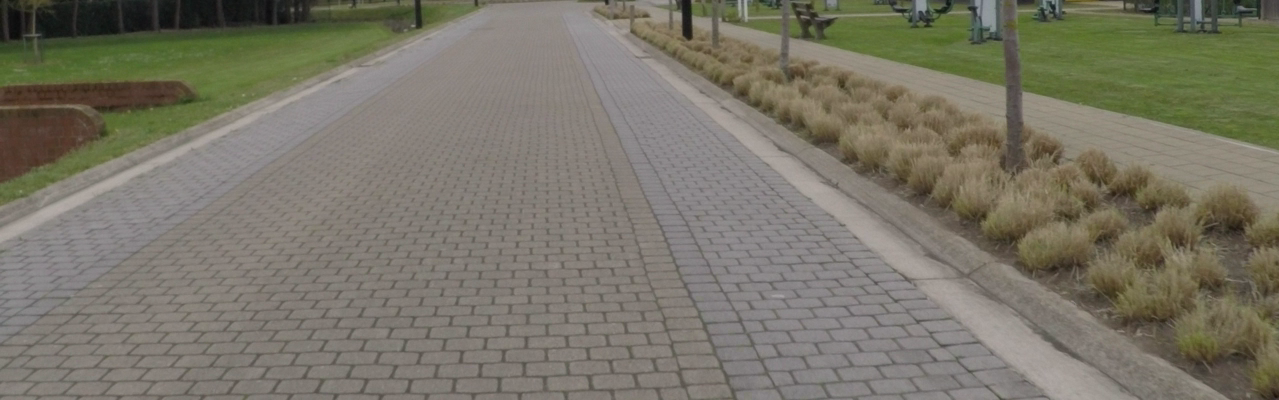
\includegraphics[width=.9\textwidth]{cobbles_in}
  \caption{Original frame\label{zebra_orig}}
\end{subfigure}%
\begin{subfigure}{.5\textwidth}
  \centering
  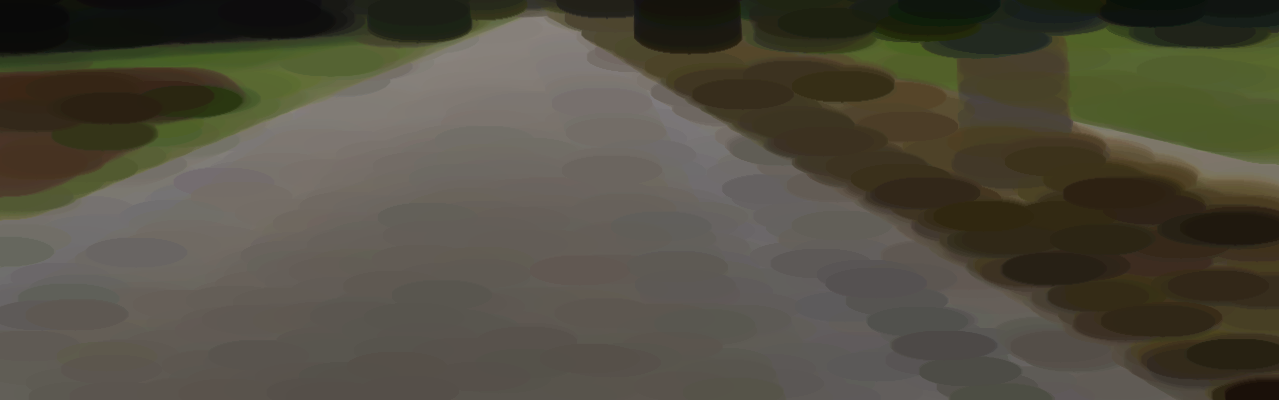
\includegraphics[width=.9\textwidth]{cobbles_erode_out}
  \caption{Objects become bigger after eroding\label{zebrawitcanny}}
\end{subfigure}
\caption{Perform eroding and dilation to remove details.}
\end{figure}


\begin{figure}[ht]
\centering
\begin{subfigure}{.5\textwidth}
  \centering
  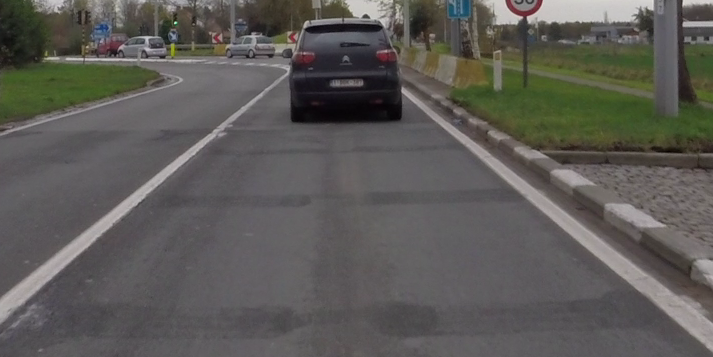
\includegraphics[width=.9\textwidth]{car_original}
  \caption{Original frame\label{zebra_orig}}
\end{subfigure}%
\begin{subfigure}{.5\textwidth}
  \centering
  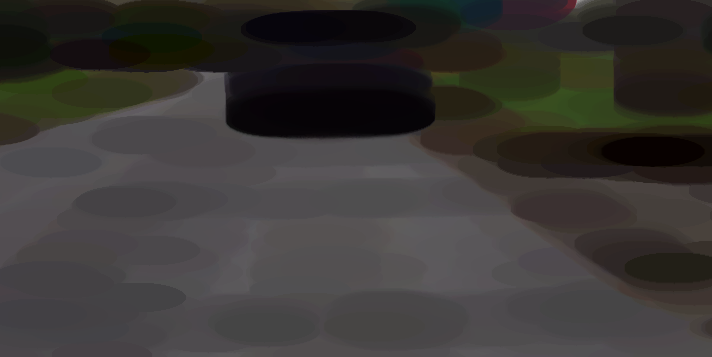
\includegraphics[width=.9\textwidth]{car_erode_bigger}
  \caption{Objects become bigger after eroding\label{zebrawitcanny}}
\end{subfigure}
\begin{subfigure}{.5\textwidth}
  \centering
  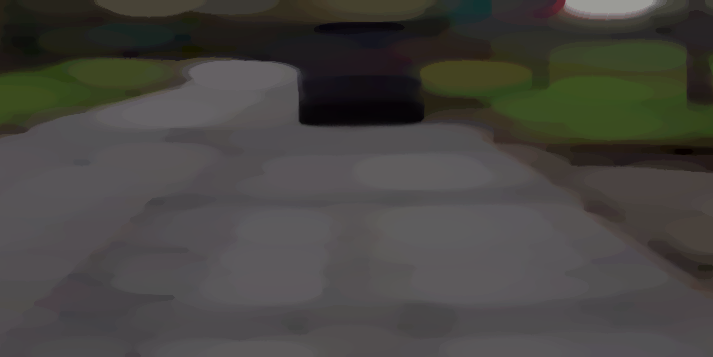
\includegraphics[width=.9\textwidth]{car_dilate_smaller}
  \caption{Restore original sizes with dilation\label{zebrawitcanny}}
\end{subfigure}
\caption{Perform eroding and dilation to remove details.}
\end{figure}


\subsection{Canny Edge Detection}